\chapter{Design Problem: An Optical Reciever}

Photonics is a relatively new field dating back to [DATE HERE]. With the increasing possibility of incorporating photonics elements on chip with the electronics, optical circuits have become a research hotspot. 

To demonstrate the capabilities of BAG, an optical reciever design from concept to verification is shown.

\section{Problem Statement and Architecture}
Photonic communication systems transmit and recieve data using light, meaning that the reciever element must be a photodiode. A reverse biased photodiode reciever element can be modeled as a current source with some capacitance in parallel. This is the ``input',' analgous to an antenna in typical RF recievers. For this design, the following arbitrary specs are required:
\begin{itemize}
\item 14nm FinFET technology
\item A data rate of 25GBps
\item A photodiode capacitance of 50fF
\item $40\mu A$ peak to peak photodiode current
\item $V_{DD}=0.8V$
\item Must use BAG for generation and the majority of testing
\end{itemize}

There are no power constraints or architecture constraints with the condition that any chosen architecture will be implemented in BAG. We will assume the photonoics are already implemented, and we will also not simulate for temperature, voltage or process variations. Noise in general should be low, but there is no strict value requirement. We will see in the ``Future Discussions'' [CHANGE THIS TO APPROPRIATE TITLE] of Chapter 5 [GET PROPER CHAPTER] how this could be extended, and an example of how one could generalize the design procedure automatically.

\subsection{Architecture Choice and Concerns}
The architecture is based off the reciever in [CITATION HERE, KRISHNA] and is shown below:
\begin{figure}[h]
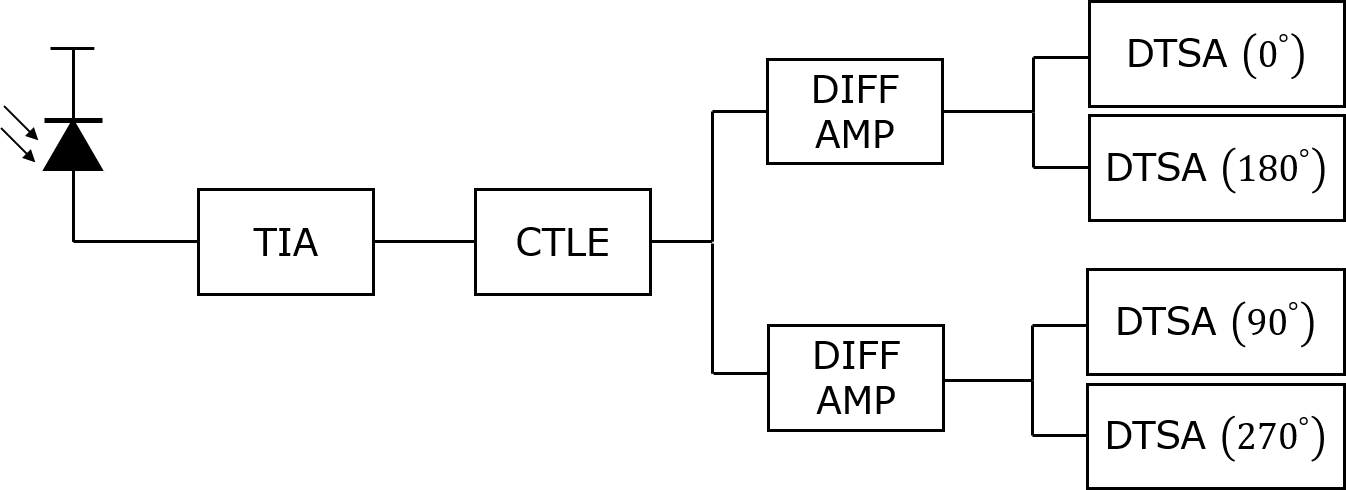
\includegraphics[width=\textwidth]{architecture}
\caption{System architecture}
\label{fig:System Architecture}
\end{figure}

This reciever is a quad data rate (QDR) reciever with each comparator operating in $90^\circ$ phase offsets at a quarter of the clock rate to reduce the comparator constraints. Technically, only a single comparator clocked at 25GHz is necessary, however the time required for a comparator to decide between a 1 or 0 bit is finite, and mostly determined by device limitations rather than designer's choice. To meet the target, we use four comparators that operate only a quarter of the time to allow enough time for decision making and regeneration.

\begin{center}
Diagram with distribution of one clock cycle vs regen + decision time goes here with some theoretical maximum ideal clock overlaid.
\end{center}

This will be further discussed in following parts of this chapter. Another design choice made is to drive the $0^\circ$ and $180^\circ$ offset comparators with the same preamp, and $90^\circ$and $270^\circ$ together. This was done to reduce the effect of back-injection of the clock into the circuit elements before it.

The transimpedance amplifier (TIA) is the main gain stage and is used to convert the incoming current waveform into a voltage. Since the TIA is the first block in the chain, the Friis formula of cascaded noise figures

\begin{equation}
\label{friis}
F_{total}=F_1+\frac{F_2-1}{G_1}+\frac{F_3-1}{G_1G_2}+...
\end{equation}

(where $F_1$ and $G_i$ are the noise factor and gain of stage $i$ respectively) tells us we want the TIA to be high gain and low noise in order to reduce the overall noise factor of the system.

The TIA is followed by a continuous time linear equalizer (CTLE). A CTLE has a zero in its transfer function that can be placed at a specific frequency, which theoretically allows the designer to extend the bandwidth of previous stages. One concern of the CTLE however, is that it can only, in general, shape the energy of the frequency spectrum. This means that usually to increase the gain at high frequency, we must throw away DC gain, as shown below:

\begin{figure}[h]
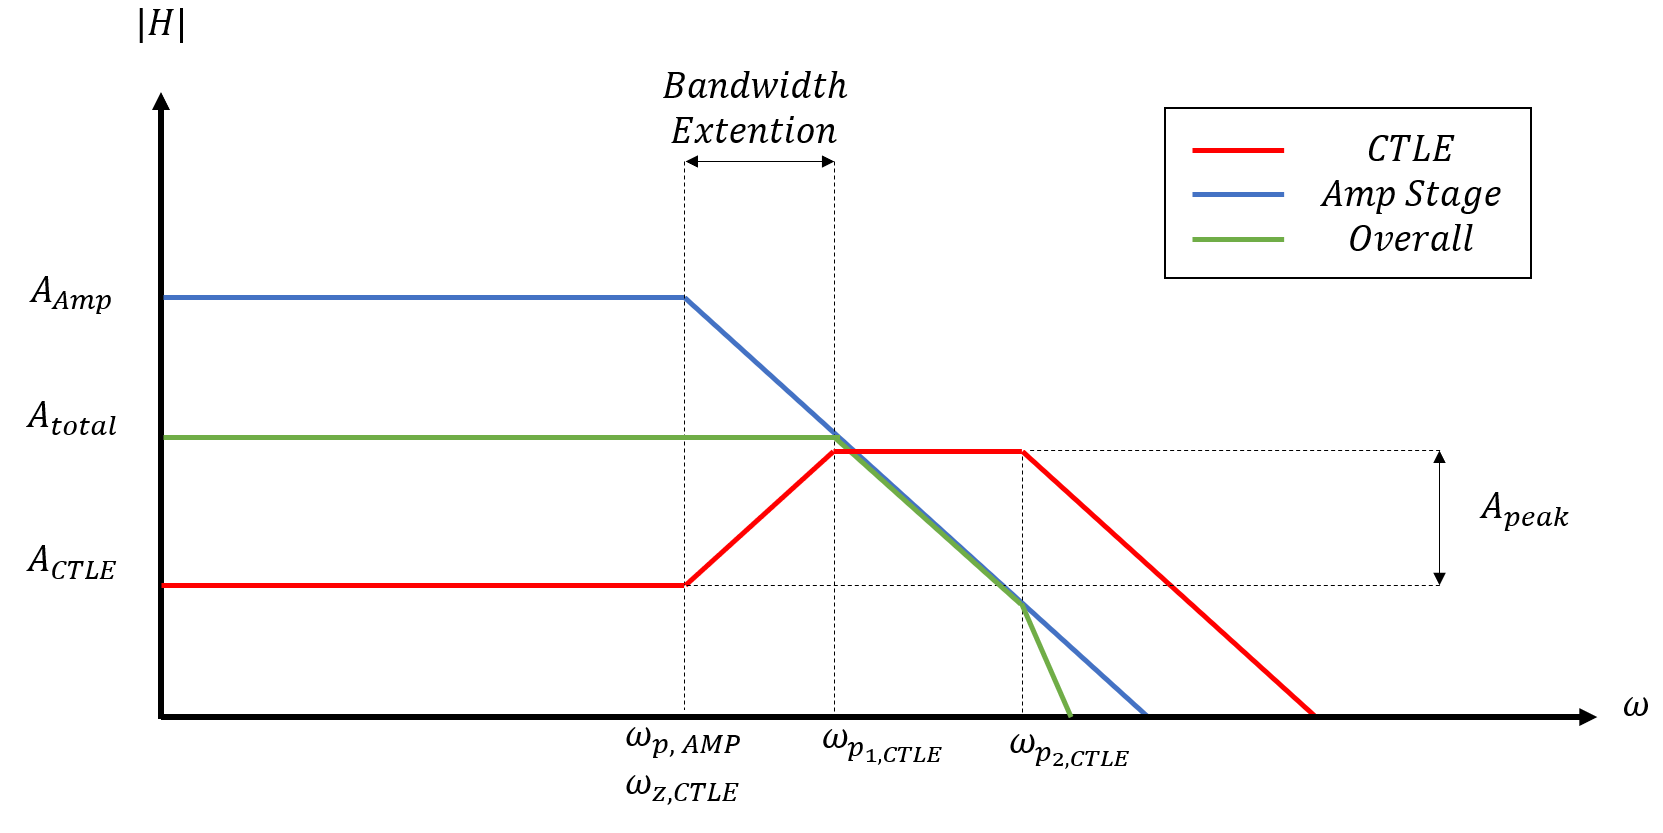
\includegraphics[width=\textwidth]{ctle_operation}
\caption{CTLE effect on a generic one-pole system}
\label{fig:CTLE Operation}
\end{figure}

Since we are targeting 25GBps, the emperical target bandwidth the front end reciever needs for a relatively optimal tradeoff in power and introduced ISI is $\approx 0.7\times$ the data rate, or roughly 17GHz [CITATION HERE]. The bare minimum would be roughly half, or 12.5GHz. We will target somewhere in between. A good rule of thumb for comparators is that they need milivolts of signal swing to consistently measure correctly. The gain bandwidth product of the TIA is unlikely to be large enough to get a $40\mu A$ signal to roughly $10mV$ across a frequency range of 0Hz to 17GHz and be low noise, so we increase the TIA gain and lower the bandwidth so that even with the CTLE DC gain reduction, we can still get decent gain in conjunction with the CTLE bandwidth extension. 

The final stage before the comparators is a set of passively loaded differential amplifiers. Their purpose is threefold. The CTLE would have to simultaneously drive four comparators, which is a fairly large capacitve load. This limits the maximum achievable peaking gain by pushing in the second pole. Additionally, the comparators tend to inject their clock signal backwards which can impact the CTLE's operation periodically. The amplifiers serve as buffers which will isolate the kickback, and act as an intermediate step to reduce the amount of capacitance the CTLE has to drive. The DC gain is also expected to be too low due to the CTLE's reduction, so the amplifiers will provide a relatively small gain ($\approx 2\times$) to get as much swing as possible.


%\begin{figure}\centering
%\parbox{.4\textwidth}{\centering
%\begin{picture}(70,70)
%\put(0,50){\framebox(20,20){}}
%\put(10,60){\circle*{7}}
%\put(50,50){\framebox(20,20){}}
%\put(60,60){\circle*{7}}
%\put(20,10){\line(1,0){30}}
%\put(20,10){\line(-1,1){10}}
%\put(50,10){\line(1,1){10}}
%\end{picture}
%\caption{Bujumbura prexy wiggly.}}
%\hfill
%\parbox{.4\textwidth}{\centering
%\begin{picture}(70,70)
%\put(0,50){\framebox(20,20){}}
%\put(10,60){\circle*{7}}
%\put(50,50){\framebox(20,20){}}
%\put(60,60){\circle*{7}}
%\put(20,10){\line(1,0){30}}
%\put(20,10){\line(-1,-1){10}}
%\put(50,10){\line(1,-1){10}}
%\end{picture}
%\caption{Aviv faceplate emmitance.}}
%\end{figure}

\section{Transimpedance Amplifier}
The TIA is implemented as a pseudo-differential structure as two CMOS inverters with resistive feedback. 
\begin{figure}[h]
\centering
\ctikzset{tripoles/mos style/arrows}
\begin{circuitikz}[american voltages]
\draw (3, 2) node[american not port](n){};
\draw (3, 3.5) node[american not port](p){};
\draw (p.out) to[short] (4, 3.5) |- (4, 4.5) to[R, l_=$R_{fb}$] (2, 4.5);
\draw (p.in) -| (2, 4.5);
\draw (n.out) to[short] (4, 2) |- (4, 1) to[R, l=$R_{fb}$] (2, 1);
\draw (n.in) -| (2, 1);
\draw (p.out) to[short, -o] (5, 3.5) to[open, v^=$V_{out}$, -o] (5, 2) to[short] (n.out);
\draw (p.in) to[short] (-1, 3.5) to[american current source, l_=$I_{DC}$] (-1, 2) to[short] (-1, 1.5) node[ground]{};
\draw (-1, 3.5) to[short, *-] (-1, 4) to[pDo] (-1, 4.5) to[short] (-1, 5) node[rground, yscale=-1]{} to[open] (-1, 5.5) node[above]{$V_{DD}$};
\draw (-1, 4.75) to[short] (0, 4.75) to[C, l=$C_{pd}$] (0, 3.5);
\draw (n.in) to[short] (1, 2) to[american current source, l_=$I_{DC}$] (1, 0.5) to[short] (1, 0) node[ground]{};
\end{circuitikz}
\label{TIA Schematic}
\caption{TIA Schematic}
\end{figure}

[CITATION HERE] about Nandish's paper with pseudo diff performance and why it was better for common mode or something.
TALK ABOUT BLEEDERS AND HOW THEY SET THE DC COMMON MODE AT THE OUTPUT.

From the small signal model (shown below) we can derive the gain and pole locations.
\begin{center}
SMALl SIGNAL MODEL + DERIVATION HERE
\end{center}

The gain is then approximately just $R_{fb}$. For a given choice of $R_{fb}$, we then use BAGs rapid iteration to sweep for transistor widths. As the size increases, device parasitics become dominant over the external capacitances, so there is an optimal size for bandwidth. Once the maximum bandwidth is found, this sets the device sizes. Since we know the CTLE can only get a couple of GHz of bandwidth extension, we sweep the TIA resistor to see what resistance gives a bandwidth of around 12GHz. This results in a gain of [GAIN GOES HERE]. If we assume the CTLE will cut the DC gain by roughly a third, and we can get about 1.5x amplification from the preamps, then the overall gain should still be high enough for the comparator.

The output common mode is set by the DC sources. Assuming $0A$ of DC current, the input common mode will be around mid-rail, so the output common mode can be approximated as follows:
\begin{equation}
\label{tia_dc}
\frac{V_{o}-\frac{V_{DD}}{2}}{R_{fb}}=I_{DC}
\end{equation}
In order to bias the CTLE input, we want this to potentially be a little higher than midrail since the $V_{GS}$ needs to be large enough to give headroom to the tail transistors. Plugging into \ref{tia_dc} gives a starting point that can then be swept using BAG for better accuracy. Post-pex hand-simulation is then used to fine tune the current the get the desired result. Note that by increasing the output common mode, the gain can reduce. This means that the resistance might need to be higher than anticipated. This is also determined by simulating BAG generated instances.

\section{Continuous Time Linear Equalizer}
A CTLE is a simple amplifier, degenerated by a parallel resistor capacitor combination as shown below:
\begin{figure}[h]
\centering
\ctikzset{tripoles/mos style/arrows}
\begin{circuitikz}[american voltages]
\draw (1, 1) node[nmos](n_in){};
\draw (3, 1) node[nmos, xscale=-1](p_in){};
\draw (n_in.drain) to[R, l=$R_d$] (1, 3.5);
\draw (1, 3.5) to[short] (2, 3.5) node[above]{$V_{DD}$};
\draw (2, 3.5) to[short] (3, 3.5) to[R, l=$R_d$] (p_in.drain);
\draw (n_in.source) to[C, *-,  l=$C_s$] (p_in.source);
\draw (n_in.source) to[short] (1, -1) to[R, *-*, l=$R_s$] (3, -1) to[short, -*] (p_in.source);
\draw (1, -2) node[nmos](n_tail){};
\draw (n_tail.drain) to[short] (1, -1);
\draw (3, -2) node[nmos](p_tail){};
\draw (p_tail.drain) to[short] (3, -1);
\draw (n_tail.source) to[short] (1, -3) to[short, -*] (2, -3) node[ground]{};
\draw (2, -3) to[short] (3, -3) to[short] (p_tail.source);
\draw (-1, -2) node[nmos, xscale=-1](bias){};
\draw (bias.source) to[short] (-1, -3) to[short] (2, -3);
\draw (bias.drain) to[short, -o] (-1, 0) node[above]{$I_{bias}$};
\draw (-1, -1) to[short, *-] (0, -1) to[short, -*] (bias.gate);
\draw (bias.gate) to[short] (p_tail.gate);
\draw (n_in.gate) node[label={[font=\footnotesize]180:$V_{in}$}] {};
\draw (p_in.gate) node[label={[font=\footnotesize]0:$V_{ip}$}] {};
\draw (p_in.drain) to[short, -o] (2.5, 1.77) to[open, v=$V_{out}$] (1.5, 1.77) to[short, o-] (n_in.drain);
\end{circuitikz}
\label{CTLE Schematic}
\caption{CTLE Schematic}
\end{figure}

Since we know the pole location of the TIA, we can design the CTLE to have its zero in close proximity. Firstly, we draw the approximate differential mode half circuit:
\begin{figure}[h]
\centering
\ctikzset{tripoles/mos style/arrows}
\begin{circuitikz}[american voltages]
\draw (1, 1) node[nmos](n_in){};
\draw (n_in.drain) to[R, l=$R_d$] (1, 3.5);
\draw (1, 3.5) node[rground, yscale=-1]{} to[open] (1, 4) node[above]{$V_{DD}$};
\draw (n_in.source) to[short] (1, 0) to[short] (0.5, 0) to[R, l_=$\frac{R_s}{2}$] (0.5, -1.5);
\draw (n_in.source) to[short] (1, 0) to[short] (1.5, 0) to[C, l=$2C_s$] (1.5, -1.5);
\draw (1.5, -1.5) to[short, -*] (1, -1.5) to[short] (0.5, -1.5);
\draw (1, -1.5) node[ground]{};
\draw (n_in.drain) to[short, -o] (1.5, 1.77)  node[label={[font=\footnotesize]0:$V_{out}$}] {};
\draw (n_in.gate) node[label={[font=\footnotesize]180:$V_{in}$}] {};
\end{circuitikz}
\label{CTLE Half-Circuit}
\caption{CTLE Half-Circuit}
\end{figure}

which by inspection, we know
\begin{equation}
\label{Gm}
G_m=\frac{g_m}{1+g_m(\frac{R_s}{2}||\frac{Z_{C_s}}{2})}
\end{equation}
\begin{equation}
G_m=\frac{2g_m(1+j\omega R_sC_s)}{2+g_mR_s+2j\omega R_sC_s}
\end{equation}
We can also determine the output impedance by inspection
\begin{equation}
\label{Ro}
R_o\approx R_l||\frac{Z_{C_l}}{2}=\frac{R_d}{1+2j\omega R_d C_l}
\end{equation}
So the overall gain is then
\begin{equation}
\label{ctle_gain}
G_mR_o=\frac{2g_m(1+j\omega R_sC_s)R_d}{(2+g_m R_s+2j\omega R_sC_s)(1+2j\omega R_dC_l)}
\end{equation}
which puts the zero at 
\begin{equation}
\label{zero}
\omega_z=\frac{1}{R_sC_s}
\end{equation}
and the first pole at 
\begin{equation}
\label{pole_1}
\omega_{p1}=\frac{1+gm\frac{R_s}{2}}{R_sC_s}
\end{equation}
with the second pole at
\begin{equation}
\label{pole_2}
\omega_{p2}=\frac{1}{2R_dC_l}
\end{equation}
and lastly, the ideal peaking gain should be 
\begin{equation}
A_{peak}=g_mR_d
\end{equation}

\section{Preamplifiers}

\section{Comparator}
The comparator usually is the first thing one would design. The comparator's limitations generally sets the required gain and noise specs for the front end. In this project, the comparator was designed last, since there is no power constraint. This means that at the cost of power, we can generally make the comparator decide between very small voltages if we are willing to burn more current.

\begin{center}
Show an equation or graph or something with the parasitic caps on the DIN/DIP nodes and how they have I+dI and I-dI going through them
\end{center}


\section{Design Verification}
